\chapter{The Necessary Google Permissions}
\label{app:GoogPerm}

%\textbf{\blfootnote{In the interest of privacy, email addresses have been changed.}}

\begin{figure}[htbp]
	\centering
	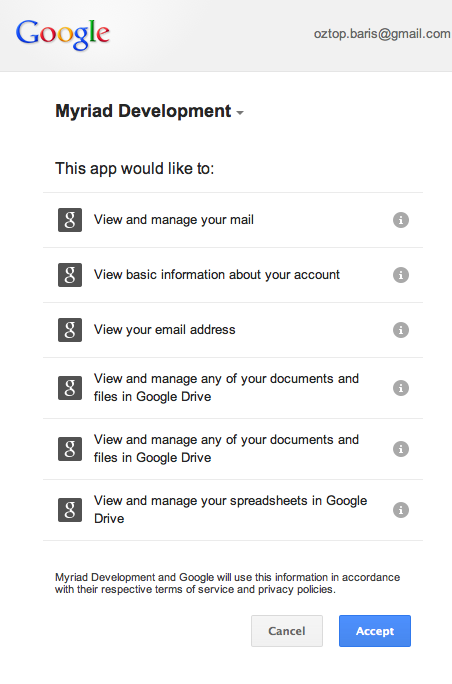
\includegraphics[scale=0.55]{imgs/GooglePermissions.png}
	\caption[The Necessary Permissions From Google to User Myriad]{The Necessary Permissions From Google to User Myriad}
	\label{fig:GooglePermissions}
\end{figure}

\begin{table}[H]
\begin{center}
	\renewcommand{\arraystretch}{1}
	%\tiny
	%\setlength{\tabcolsep}{5pt}
	\caption[Comparison Matrix for Help Desk Applications]{Comparison Matrix for Help Desk Applications} \label{tab:comp_matr_help}
    \begin{tabular}{ | p{5cm} | p{8cm} | }
	\hline
	\textbf{Permission} & \textbf{Description} \\ \hline
	\textbf{View and manage your mail} & 
	\begin{compactitem}
		\item View and manage your mail in Google Mail
	\end{compactitem} \\ \hline
	\textbf{View basic information about your account} &
	\begin{compactitem}
		\item View your name, public profile URL, and photo
		\item View your gender and birthdate
		\item View your country, language, and timezone
	\end{compactitem} \\ \hline
	\textbf{View your email address} &
	\begin{compactitem}
		\item View the email address associated with your account
	\end{compactitem} \\ \hline
	\textbf{View and manage any of your documents and files in Google Drive} &
	\begin{compactitem}
		\item List and search all of your documents and files in Google Drive
		\item Download any of your documents and files in Google Drive
		\item Create, move, copy, edit, or delete any of your documents and files in Google Drive
		\item Share or unshare any of your documents and files in Google Drive
	\end{compactitem} \\ \hline
	\textbf{View and manage any of your documents and files in Google Drive} &
	\begin{compactitem}
		\item List and search all of your documents and files in Google Drive
		\item Download any of your documents and files in Google Drive
		\item Create, move, copy, edit, or delete any of your documents and files in Google Drive
		\item Share or unshare any of your documents and files in Google Drive
	\end{compactitem} \\ \hline
	\textbf{View and manage your spreadsheets in Google Drive} &
	\begin{compactitem}
		\item Create new spreadsheets
		\item View and modify existing spreadsheets
		\item Share spreadsheets with others
	\end{compactitem} \\ \hline	
    \end{tabular}
\end{center}
\end{table}